% Degrees of freedom needed for the first 1000 eigenvalues: the largest relative
% error over the block against the degrees of freedom, one curve per
% discretisation, with the tolerances as levels and the extrapolations beyond the
% sweep as dotted continuations. Right isosceles triangle domain.
%
% The reference is the closed form of the spectrum, so there is no reference
% floor here and none is drawn; on the L-shape, whose reference is a DST run,
% there is one.
%
% Requires in the preamble:
%   \usepackage{graphicx}
%   \usepackage{epstopdf}   % the figure is EPS; needed under pdflatex,
%                           % which then wants -shell-escape. Not needed for
%                           % latex/dvips, which reads EPS directly.
%
% The figure lives next to this file, in results/eigenvalues_dof_requirement/.
% If you \input this snippet from elsewhere, point graphicx at that folder, e.g.
%   \graphicspath{{results/eigenvalues_dof_requirement/}}
% and drop the leading path from the \includegraphics argument below.

\begin{figure}[htbp]
  \centering
  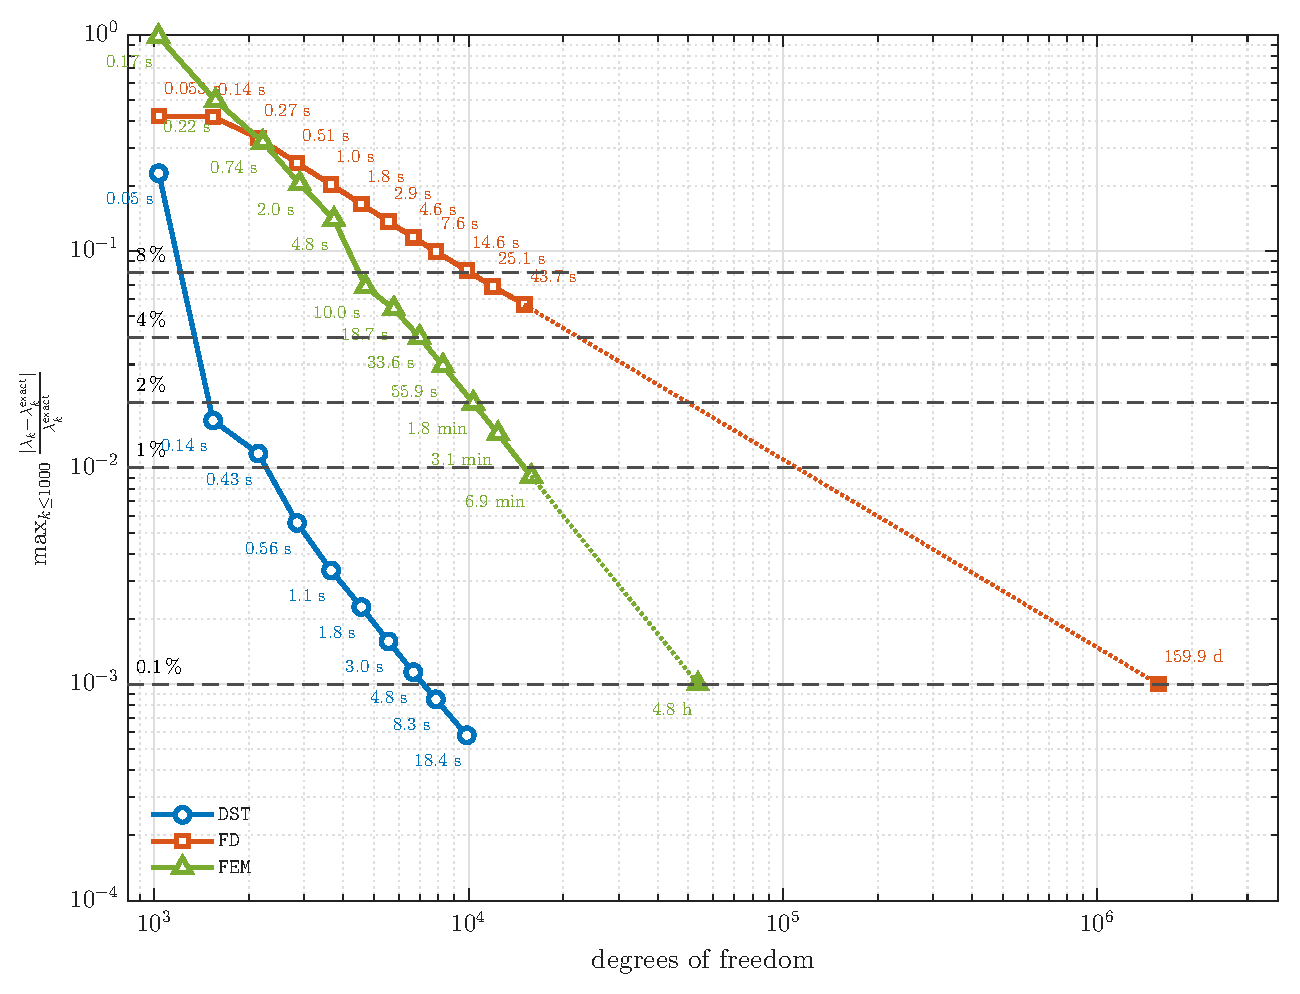
\includegraphics[width=0.85\textwidth]{isosceles_triangle_dof_requirement_n1000}
  \caption{Accuracy of the first 1000 eigenvalues of Laplace operator, zero Dirichlet boundary conditions, right isosceles triangle domain \texttt{isosceles\_triangle}. Largest relative error over the whole block of first $1000$ eigenvalues, $\left\{ \lambda_k \right\}_{k=1}^{1000}$, $\max_{k \leq 1000} \frac{|\lambda_k - \lambda_k^{\text{exact}}|}{\lambda_k^{\text{exact}}}$, against the degrees of freedom used by each discretisation of Laplace operator, compared with the exact eigenvalues $\lambda_{m,n} = m^2 + n^2$, $m > n \geq 1$, of the continuous eigenvalue problem; \texttt{FEM} -- finite element method, \texttt{FD} -- finite differences method, \texttt{DST} -- discrete sine transform method. Each marker is labelled with the computation time of the particular run, dotted lines show extrapolated values.}
  \label{fig:dof_requirement_isosceles_triangle}
\end{figure}
